\documentclass[12pt,a4paper]{article}

\usepackage[a4paper,text={16.5cm,25.2cm},centering]{geometry}
\usepackage{lmodern}
\usepackage{amssymb,amsmath}
\usepackage{bm}
\usepackage{graphicx}
\usepackage{microtype}
\usepackage{hyperref}
\usepackage{minted}
\setlength{\parindent}{0pt}
\setlength{\parskip}{1.2ex}

\hypersetup
       {   pdfauthor = {  },
           pdftitle={  },
           colorlinks=TRUE,
           linkcolor=black,
           citecolor=blue,
           urlcolor=blue
       }






\begin{document}



\section{Aproksimacija z linearnim modelom}
Podatke ${(x_1,y_1),(x_2,y_2),...,(x_n,y_n)}$ želimo opisati s funkcijo oblike $y = f(x,p)$ Delali bomo s podatki CO2 na Mauna Loa Potrebno je prebrati podatke iz podatkovne baze in jih pripraviti za delo.


\begin{minted}[texcomments = true, mathescape, fontsize=\small, xleftmargin=0.5em]{julia}
using FTPClient
using Statistics
url = "ftp://aftp.cmdl.noaa.gov/products/trends/co2/co2_weekly_mlo.txt"
io = download(url)
data = readlines(io)

using Plots
filter!(l->l[1]!='#', data)
data = strip.(data)
data = [split(line, r"\s+") for line in data]
data = [[parse(Float64, x) for x in line] for line in data]
filter!(l->l[5]>0, data)
data_4 = [l[4] for l in data]
t0 = mean(data_4)
t1 = [l[4] for l in data]
t = [l[4] - t0 for l in data] 
co2 = [l[5] for l in data]
\end{minted}
\begin{minted}[texcomments = true, mathescape, fontsize=\small, xleftmargin=0.5em, frame = leftline]{text}
2584-element Vector{Float64}:
 333.37
 332.95
 332.35
 332.2
 332.37
 331.73
 331.69
 331.46
 330.83
 330.76
   |$\ensuremath{\vdots}$|
 422.28
 425.83
 423.54
 425.21
 425.13
 425.45
 425.74
 425.37
 425.04
\end{minted}

Graf 1


\begin{minted}[texcomments = true, mathescape, fontsize=\small, xleftmargin=0.5em]{julia}
scatter(t1, co2, title="Atmosferski CO2 na Mauna Loa",
        xlabel="leto", ylabel="parts per milion (ppm)", label="co2",
        markersize=1)
\end{minted}
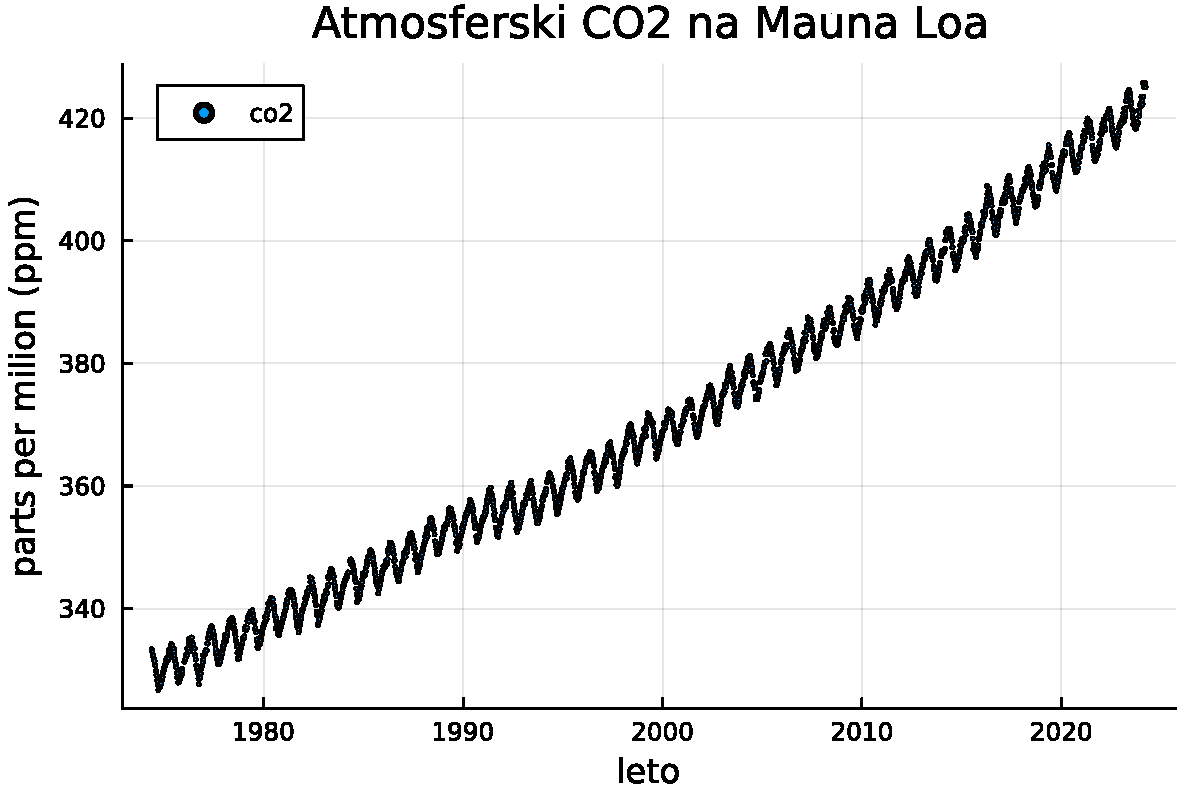
\includegraphics[width=\linewidth]{jl_AuRI8c/demo_2_1.pdf}

Glede na podatke izračunamo letne spremembe CO2


\begin{minted}[texcomments = true, mathescape, fontsize=\small, xleftmargin=0.5em]{julia}
using LinearAlgebra
A = hcat(ones(size(t)), t, t.^2, cos.(2pi*t), sin.(2pi*t))
p = A\co2 #co2 = y
norm(A*p-co2)
\end{minted}
\begin{minted}[texcomments = true, mathescape, fontsize=\small, xleftmargin=0.5em, frame = leftline]{text}
53.84978787225933
\end{minted}

Graf 2


\begin{minted}[texcomments = true, mathescape, fontsize=\small, xleftmargin=0.5em]{julia}
plot([A[:,1]/norm(A[:,1]), A[:,2]/norm(A[:,2]), A[:,3]/norm(A[:,3])], ylims=[0,0.025], title="Normirani stolpci matrike A")
\end{minted}
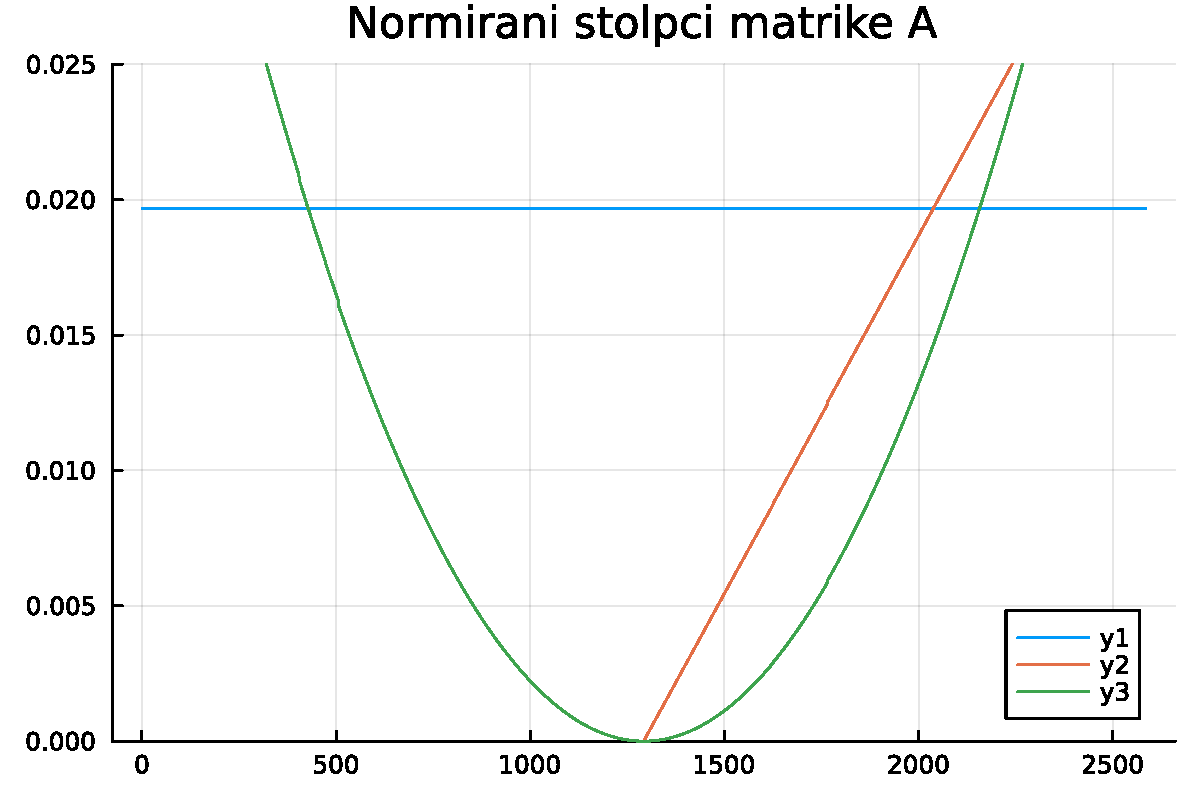
\includegraphics[width=\linewidth]{jl_AuRI8c/demo_4_1.pdf}

Graf 3


\begin{minted}[texcomments = true, mathescape, fontsize=\small, xleftmargin=0.5em]{julia}
plot(t, p[2].+2*p[3]*(t), title="Letne spremembe CO2", xaxis=[1980,1990,2000,2010,2020])

model(t) =  p[1]+ p[2]*(t-t0) + p[3]*(t-t0)^2 + p[4]*cos(2*pi*t) + p[5]*sin(2*pi*t)
model.([2020, 2030, 2050])
\end{minted}
\begin{minted}[texcomments = true, mathescape, fontsize=\small, xleftmargin=0.5em, frame = leftline]{text}
3-element Vector{Float64}:
 414.5937232610704
 440.1696411434572
 499.7031888979348
\end{minted}

Graf napovedi


\begin{minted}[texcomments = true, mathescape, fontsize=\small, xleftmargin=0.5em]{julia}
plot(model.([2020,2030,2050]))
\end{minted}
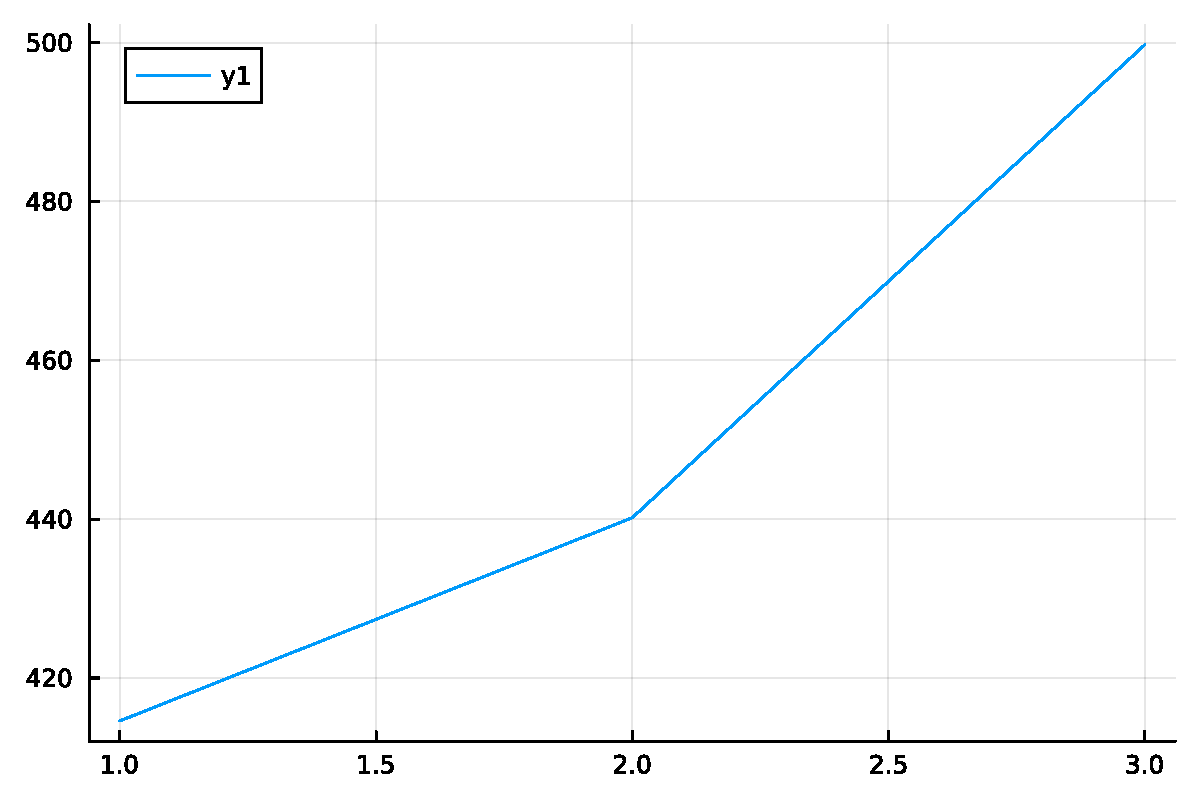
\includegraphics[width=\linewidth]{jl_AuRI8c/demo_5_1.pdf}


\end{document}
